\chapter{Preliminaries}  \label{chap:Prel}
%%%%%%%%%%%%%%%%%%%%%%%%%%%%%%%%%%%%%%%%%%%%%%%%%%%%%%%%%%

In this chapter, we introduce  some notation and results used throughout our presentation. We also introduce the concept of risk measure that will be used in Chapter \ref{chap:App}.

\section{Basic results}

First we  consider the  index set  ${\mathbb{N}}:=\{0,1,2,\ldots\}$,  the usual inner  product  $\langle \cdot,\cdot \rangle$ in $\mathbb{R}^n$, and the associated Euclidean norm    $\|\cdot\|$.
Let  $f:\mathbb{R}^n \to \mathbb{R}$ be a differentiable function and $C \subseteq \mathbb{R}^n$. The  gradient $\nabla f$ of $f$ is said to be {\it Lipschitz continuous} in $C$ with constant $L>0$ if $\|\nabla f(x)-\nabla f(y)\|\leq L \|x-y\|$, for all~$x, y\in C$. Combining this definition with the fundamental theorem of calculus, we obtain the following result whose proof can be found in \cite[Proposition A.24]{Bertsekas1999}.

\begin{lemma} \label{Le:derivlipsch}
	Let $f:\mathbb{R}^n \to \mathbb{R}$ be a differentiable function and $C \subseteq \mathbb{R}^n$. Assume that $\nabla f$  is Lipschitz continuous in C with constant $L>0$. Then,
	\[
		f(y) - f(x) - \langle \nabla f(x), y-x \rangle \leq (L/2)\|x-y\|^2,
	\]
	for all~ $x, y\in C$.
\end{lemma}
%Let $f:\mathbb{R}^n \to \mathbb{R}$ be a differentiable function and $C \subseteq \mathbb{R}^n$ be a convex set. The function $f$ is convex on $C$, if $f(y) \geq  f(x) + \langle \nabla f(x), y-x \rangle$, for all $x, y\in C$.
Assume that $C$ is a convex set. The function $f$ is said to be \textit{convex} on $C$, if
\[
	f(y) \geq  f(x) + \langle \nabla f(x), y-x \rangle,
\]
for all $x, y\in C$. We recall  that a point ${\bar{x}} \in C$ is a {\it stationary point} for problem \eqref{eq:OptP} if
\begin{equation} \label{eq:StatPoint}
	\langle \nabla f({\bar{x}}),  x-{\bar{x}}\rangle \geq 0, \qquad \forall ~ x\in  C.
\end{equation}
Consequently, if $f$ is a convex funct{}ion  on $C$, then  \eqref{eq:StatPoint} implies that  $\bar{x} \in \Omega^*$.  We will now present some useful concepts  for the analysis of the sequence generated by the scaled  gradient method, for more details, see \cite{CombettesVu2013}.    For that,  let  $D$ be a $n\times n$ positive definite matrix and $\| \cdot \|_{D} : \mathbb{R}^{n}\rightarrow \mathbb{R}$ be  the norm  defined by
\begin{equation} \label{def:normaD}
	\|d\|_{D}:=\sqrt{\left\langle D d,d\right\rangle},\quad \forall d\in \mathbb{R}^{n}.
\end{equation}
For a fixed  constant $\mu \geq 1$,  {\it denote by  ${\cal D}_{\mu}$  the set of symmetric positive definite matrices $n\times n$ with all eigenvalues contained in the interval $[\frac{1}{\mu}, \mu]$}.  The set ${\cal D}_{\mu}$   is compact. Moreover,  for each $D\in {\cal D}_{\mu}$, it follows that $D^{-1}$ also belongs to $ {\cal D}_{\mu}$. Furthermore,  due to $D\in {\cal D}_{\mu}$,  by \eqref{def:normaD}, we obtain
\begin{equation} \label{eq:pnv}
	\frac{1}{\mu}\|d\|^2\leq \|d\|^2_{D}\leq \mu \|d\|^2, \qquad \forall d\in \mathbb{R}^n.
\end{equation}

Let us recall the the concept of  sequence  quasi-Fej\'er  monotone to a set, introduced in  \cite{CombettesVu2013}.
\begin{definition} \label{def:QuasiFejer}
	Let $(y^k)_{k\in\mathbb{N}}$ be a sequence in $\mathbb{R}^n$ and   $(D_k)_{k\in\mathbb{N}}$ be  a sequence in ${\cal D}_{\mu}$.  The sequence $(y^k)_{k\in\mathbb{N}}$ is said to be quasi-Fej\'er  monotone to a set $W\subset \mathbb{R}^n$ with respect to  $(D_k)_{k\in\mathbb{N}}$ if, there exists  a sequence $(\eta_k)_{k\in\mathbb{N}}\subset [0, +\infty)$ such that $\sum_{k\in \mathbb{N}}\eta_k<\infty$ and for  all $w\in W$, there exists a sequence $(\epsilon_k)_{k\in\mathbb{N}}\subset[0, +\infty)$ such that  $\sum_{k\in \mathbb{N}}\epsilon_k<\infty$, and
	\[
		\|y_{k+1}-w\|_{D_{k+1}}^2\leq (1+\eta_k) \|y^k-w\|_{D_k}^2+\epsilon_k,
	\]
	for    all $k\in \mathbb{N}$.
\end{definition}

The following lemma is useful to study the  quasi-Fej\'er  monotone sequence, its prove can be found in \cite[Lemma 2.2.2]{PolyakLivro1987}.
\begin{lemma} \label{le:pl}
	Let $(\alpha_k)_{k\in\mathbb{N}}$, $(\eta_k)_{k\in\mathbb{N}}$ and $(\epsilon_k)_{k\in\mathbb{N}}$ be a sequences in $[0, +\infty)$  such that $\sum_{k\in \mathbb{N}}\eta_k<\infty$ and $\sum_{k\in \mathbb{N}}\epsilon_k<\infty$. Assume that $\alpha_{k+1}\leq (1 +\eta_k)\alpha_k+\epsilon_k$, for all $k\in {\mathbb N}$. Then, $(\alpha_k)_{k\in\mathbb{N}}$ converges.
\end{lemma}

The main property of  quasi-Fej\'er  monotone sequences is stated in the following. Its proof can be found in \cite[Proposition~3.2 and Theorem 3.3]{CombettesVu2013}. For sake of completeness, we include it here.

\begin{theorem}\label{teo.qf}
	Let $(y^k)_{k\in\mathbb{N}}$ be a sequence in $\mathbb{R}^n$ and   $(D_k)_{k\in\mathbb{N}}$ be  a sequence in ${\cal D}_{\mu}$ such that $\lim_{k\rightarrow\infty}D_k={\bar D}$.   If $(y^k)_{k\in\mathbb{N}}$ is quasi-Fej\'er  monotone to a nonempty set $W\subset  \mathbb{R}^n$ with respect to $(D_k)_{k\in\mathbb{N}}$ then,  for each  $w\in W$,    the sequence  $(\|y^{k}-w\|_{D_{k}})_{k\in\mathbb{N}}$ converges. Furthermore, $(y^k)_{k\in\mathbb{N}}$ is bounded and, if each  cluster point of $(y^k)_{k\in\mathbb{N}}$ belongs to $W$, then there exists ${\bar y}\in W$ such that $\lim_{k\rightarrow\infty}y^k={\bar y}$.
\end{theorem}

\begin{proof}
	Take $w\in W$ and define the sequence $(\alpha_k)_{k\in\mathbb{N}}$, where $\alpha_k:=\|y^{k}-w\|_{D_{k}}$. Since $(y^k)_{k\in\mathbb{N}}$ is quasi-Fej\'er  monotone to $W$, Lemma~\ref{le:pl} implies that $(\alpha_k)_{k\in\mathbb{N}}$ converges. Now, by using  the  first  inequality in \eqref{eq:pnv}, we have  $\|y^{k}-w\|\leq \sqrt{\mu} \alpha_k$, for all $k\in  \mathbb{N}$.  Thus, $(y^k)_{k\in\mathbb{N}}$ is bounded. To prove the last statement, assume that   ${\bar y}, {\hat y} \in  W$   are  cluster points of $(y^k)_{k\in\mathbb{N}}$, and set   $(y^{k_i})_{i\in\mathbb{N}}$ and  $(y^{k_j})_{j\in\mathbb{N}}$  subsequences  of $(y^k)_{k\in\mathbb{N}}$ such that $\lim_{j\to +\infty} y^{k_i} = {\bar y}$ and $\lim_{j\to +\infty} y^{k_j} = {\hat y}$. It follows from the first statement that  $(\|y^{k}- {\bar y}\|_{D_{k}})_{k\in\mathbb{N}}$ and  $(\|y^{k}- {\hat y}\|_{D_{k}})_{k\in\mathbb{N}}$ are convergent. Since $\lim_{k\rightarrow\infty}D_k={\bar D}$, we have  $\lim_{k\rightarrow\infty}\|{\bar y}\|_{D_k}={\|\bar y}\|_{{\bar D}}$ and $\lim_{k\rightarrow\infty}\|{\hat y}\|_{D_k}={\|\hat y}\|_{{\bar D}}$. Hence,  due~to
	$$
		\langle y^k,  D_k({\bar y}- {\hat y})\rangle=\frac{1}{2}(\|y^{k}- {\hat y}\|_{D_{k}}^2-\|y^{k}- {\bar y}\|_{D_{k}} +\| {\bar y}\|_{D_{k}}-\| {\hat y}\|_{D_{k}}),
	$$
	for all $k\in {\mathbb N},$ we conclude that the sequence  $(\langle  y^k,  D_k({\bar y}- {\hat y})\rangle)_{k\in\mathbb{N}}$ converges.  Thus, taking into account that   $\lim_{j\to +\infty} y^{k_i} = {\bar y}$, $\lim_{j\to +\infty} y^{k_j} = {\hat y}$ and  $\lim_{k\rightarrow\infty}D_k={\bar D}$ we obtain that
	$$
		\langle  {\bar y},  {\bar D}({\bar y}- {\hat y})\rangle=\lim_{i\rightarrow\infty} \langle y^{k_i},  D_{k_i}({\bar y}- {\hat y})\rangle=\lim_{j\rightarrow\infty} \langle y^{k_j},  D_{k_j}({\bar y}- {\hat y})\rangle= \langle  {\hat y},  {\bar D}({\bar y}- {\hat y})\rangle.
	$$
	Hence, using \eqref{eq:pnv}, we obtain
	$$
		\frac{1}{\mu}\|{\bar y}- {\hat y}\|^2\leq  \|{\bar y}- {\hat y}\|^2_{\bar D}=  \langle  {\bar y},  {\bar D}({\bar y}- {\hat y})\rangle-  \langle  {\hat y},  {\bar D}({\bar y}- {\hat y})\rangle=0,
	$$
	which implies that ${\bar y}= {\hat y}$. Therefore, due to  $(y^k)_{k\in\mathbb{N}}$ be bounded, we conclude that    $(y^k)_{k\in\mathbb{N}}$ converges to ${\bar y}$.
\end{proof}

\section{Risks measures}

In the world of investments, one of the main points to be observed is the risk of an asset, that is, the possibility of losing money investing in this asset. Off course, there are \textbf{risk free} assets, where there is no possibility of losing money investing in this assets, like Treasury Bonds. The reason that leads an investor to choose a risky asset is the expectation of earning a higher return that overcomes the possibility of losing money.

We consider a universe of $n$ assets, and define how the capital will be divided in this assets.

\begin{definition}
	A portfolio with $n$ assets, $A1, A2, \dots, An$, is a vector $x^\top = (x_1, x_2, \dots, x_n)$ where each coordinate $x_i$ is the weight of capital invested in asset $Ai$.
\end{definition}

We assume that the capital is fully allocated, that is,
$$
	\sum_{i=1}^n x_i = \textbf{1}^\top x=1,
$$
where $ \mathbf{1}^\top= (1,1,\dots,1)$. Furthermore, we consider $x_i\geq 0$ for all $i$, this means that the investor cannot ``\textit{sell without having}'' an asset in the portfolio.\footnote{At first glance, it may seem strange the possibility of an investor selling a good that he does not own, but this practice is common in the market and is called \textbf{short sale}.}


There are many strategies to allocate capital in a portfolio, some of them are based in to limit the portfolio risk. To study this strategies we need to define a risk measure. In 1999 Artzner, Delbaen, Eber and Heath (see in \cite{Artzner1999}) defined that, in order for a function $\mathcal{R}(x)$ to be considered a \emph{coherent risk measure}, it needs to satisfy four properties:

\begin{enumerate}
	\item Subadditivity

	      \[
		      \mathcal{R}(x_1+x_2) \leq \mathcal{R}(x_1) + \mathcal{R}(x_2),
	      \]

	      that is, joining two portfolios into one is less risky than keeping them
	      separated.


	\item Homogeneity
	      \[
		      \mathcal{R}(\lambda x) = \lambda \mathcal{R}(x), \qquad \mbox{se } \lambda
		      \geq 0.
	      \]

	      This property ensures that leverages (borrowing to invest) affect risk proportionately.

	\item Monotonicity
	      \[
		      \mbox{if } x_1 \prec x_2, \qquad \mbox{then } \mathcal{R}(x_1) \leq \mathcal{R}(x_2).\\
	      \]

	      If a portfolio $x_1$ performs worse than $x_2$ in any
	      scenario $(x_1 \prec x_2)$, then it means that the portfolio $x_1$ is
	      riskier than $x_2$.

	\item Translation
	      \[
		      \mbox{if } m\in\mathbb{R}, \mbox{then } \mathcal{R}(x+m) = \mathcal{R}(x)-m.
	      \]
	      Adding an amount of cash, $m$, to a portfolio decreases your risk by the same amount.
\end{enumerate}


In 2002, Föllmer and Shield (see in \cite{Follmer2002}) proposed a version replacing the
homogeneity and subadditivity, by convexity:
\[
	\mathcal{R}(\lambda x_1 + (1-\lambda)x_2) \leq \lambda \mathcal{R}(x_1) + (1-\lambda) \mathcal{R}(x_2).
\]
This condition tells us that diversification does not increase risk.\footnote{Note that a function satisfying conditions 1 and 2 is convex, otherwise is not true. So this is a weaker version.}

Before we look at which functions meet the four conditions above,
we will introduce some important concepts in the study of portfolios.

A portfolio with $n$ assets, $A1, A2, \dots, An$, is a vector of the type
$x^\top = (x_1, x_2, \dots, x_n)$ where each coordinate $x_i$ is the
proportion of the capital invested in the asset $Ai$. We will assume that the capital
is fully allocated, that is, $\sum_{i=1}^n x_i = \textbf{1}^\top x=1$, where
$ \mathbf{1}^\top= (1,1,\dots,1)$. Furthermore, we will consider $x_i\geq 0$ for all $i$, this means that the investor cannot ``\textit{sell without having}'' an asset in the portfolio.\footnote{It may seem strange the possibility of an investor selling a good that he does not own, but this practice is common in the market and is called \textbf{short sale}.}


We denote by $R^\top = (R_1, R_2, \dots R_n)$ the vector of asset returns, where $R_i$ is the return on assets $i$. It follows that the return of portfolio $x$ is $R(x) = \sum_{i=1}^n x_i R_i$, we can also write in matrix form, $R(x) = x^\top R$.

Let $\mu = \mathbb{E}[R]$ be the vector of expected returns and $\Sigma = [(R-\mu)(R-\mu)^\top]$ the covariance matrix of asset returns. The expected return of portfolio is

\[
	\begin{aligned}
		\mu(x) & = \mathbb{E}[R(x)]=\mathbb{E}[x^\top R] = x^\top \mathbb{E}[R] \\
		       & = x^\top \mu,
	\end{aligned}
\]

and its variance is equal to

\[
	\begin{aligned}
		\sigma^2 & = \mathbb{E}\Big[\Big(R(x)-\mu(x)\Big)\Big(R(x)-\mu(x)\Big)^\top\ \Big]                        \\
		         & = \mathbb{E}\Big[\Big(x^\top R - x^\top \mu \Big)\Big(x^\top R - x^\top \mu \Big)^\top \ \Big] \\
		         & = \mathbb{E}\Big[x^\top(R-\mu)(R-\mu)^\top x \Big]                                             \\
		         & = x^\top \mathbb{E}\Big[(R-\mu)(R-\mu)^\top \Big] x                                            \\
		         & = x^\top \Sigma x.
	\end{aligned}
\]
The variance (or standard deviation) of an asset returns is called \textbf{volatility} of the asset.

By definition, the loss of a portfolio is $L(x) = -R(x)$, so we can define different risk measures:

\begin{itemize}
	\item Volatility of the loss:
	      \[
		      \mathcal{R}(x) = \sigma(L(x)) =\sigma(-R(x)) = \sigma (x).
	      \]
	      The standard deviation of loss was defined as a measure of risk to a portfolio by Nobel laureate in economics, Harry
	      Markowitz in 1952 (see in \cite{Markowitz1952}).

	\item VaR (Value at Risk):
	      \begin{equation}\label{eq:var}
		      \mathcal{R}(x) = \mbox{VaR}_\alpha(x) = \inf\{\ell\in\mathbb{R} : P[L(x)\leq \ell]\geq \alpha \},
	      \end{equation}
	      where $0<\alpha<1$ and $P[L(x)\leq \ell]$ is the probability of loss $L(x)$ being less than $\ell$. The Value at Risk, VaR$_\alpha$, is the $100\alpha-$percentile of loss distribution, that is, the probability of loss being less than the VaR$_\alpha$ is $\alpha$.

	      % The example below shows that in 95\% of cases, losses will be less than VaR$_{95\%}$.

	      % \begin{figure}[!h]
	      % \centering
	      % 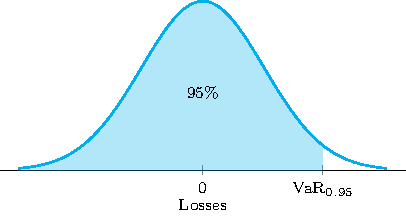
\includegraphics[width=0.5\textwidth]{figures/VaR}
	      % \caption{VaR$_{95\%}$ as the 95th percentile of the loss distribution.}
	      % \end{figure}

	\item CVaR (Conditional Value at Risk):\footnote{CVaR is also known
		      \emph{Expected Shortfall}.}

	      \begin{equation*}
		      \mathcal{R}(x) =\mbox{ES}_\alpha (x) = \mathbb{E}[L(x)|L(x)\geq \mbox{VaR}_\alpha(x)]
	      \end{equation*}
	      The CVaR, $\mbox{ES}_\alpha (x)$, is the expected value of loss, when it is grater than $\mbox{VaR}_\alpha$,
	      \begin{equation}
		      \mbox{ES}_\alpha(x) = \frac{1}{1-\alpha}\int_{\mbox{\footnotesize{VaR}}_\alpha(x)}^\infty u p(u)du
	      \end{equation}
	      where $p(u)$ is the probability density function of loss. CVaR quantifies the average loss above $\mbox{VaR}_\alpha$.

	      % The figure below shows the region where the CVaR is calculated.
	      % \begin{figure}[!h]
	      % \centering
	      % 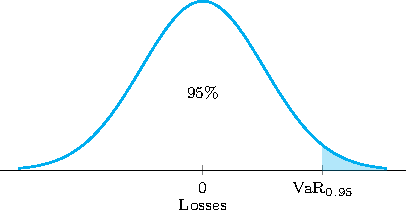
\includegraphics[width=0.5\textwidth]{figures/CVaR}
	      % \caption{Loss values used in CVaR calculation.}
	      % \end{figure}
\end{itemize}

While VaR answers the following question:

``\textit{What is the minimum portfolio loss in the $100(1-\alpha)$\% worst case scenarios}?''


CVaR answers the following question:

``\textit{What is the average loss of the portfolio in the $100(1-\alpha)$\% worst case scenarios?}''

\begin{remark}\normalfont \hspace{1cm}
	\begin{itemize}
		\item The standard deviation does not satisfy condition 4, however, this condition was defined with the perspective of banking system risk and is often ignored in case of portfolio construction.
		\item VaR is not a coherent risk measure as it does not satisfy condition 1. This is a problem because the portfolio’s risk may have be meaningful in this case.
		\item CVaR is a coherent risk measure.
	\end{itemize}
\end{remark}


Let us now assume that the returns are normally distributed, that is, $R\sim N(\mu,\sigma^2)$, where $\mu(x)=x^\top\mu$ and
$\sigma(x)=\sqrt{x^\top \Sigma x}$. Let $\phi(z) = \frac{1}{\sqrt{2\pi}}e^{-z^2/2}$ be the probability density function of Standard Normal Distribution and $\Phi(x) = \int_{-\infty}^{x}\phi(z) dz$
the standard normal accumulated density function.

By definition we have
$P\Big[L(x)\leq \mbox{VaR}_\alpha(x)\Big]=\alpha$, so
$P\Big[R(x)\leq -\mbox{VaR}_\alpha(x)\Big]=1-\alpha$, which standardizing
we have:
\[
	P\left[ \frac{R(x)-x^\top\mu}{\sqrt{x^\top \Sigma x}} \leq \frac{-\mbox{VaR}_\alpha(x)- x^\top\mu}{\sqrt{x^\top \Sigma x}}
		\right]=1-\alpha.
\]
Hence,
\[
	\frac{-\mbox{VaR}_\alpha(x)-x^\top\mu}{\sqrt{x^\top \Sigma x}}=\Phi^{-1}(1-\alpha)
\] and since $\Phi^{-1}(\alpha)=-\Phi^{-1}(1-\alpha)$, we have
\begin{equation}\label{eq:var2}
	\mbox{VaR}_\alpha(x)=-x^\top\mu+ \Phi^{-1}(\alpha)\sqrt{x^\top \Sigma x}.
\end{equation}

This is a special case of the standard deviation-based risk measure with $c = \Phi^{-1} (\alpha)$. It implies that the value-at-risk is a coherent and convex risk measure if the asset returns are normally distributed. The expression of the expected shortfall is:

\[
	\mbox{ES}_\alpha(x) = \frac{1}{1-\alpha}\int_{\mbox{VaR}_\alpha(x)}^\infty u p(u)du,
\] considering $p(u)$ the normal density function, we have that:
\[
	\mbox{ES}_\alpha(x) = \frac{1}{1-\alpha}\int_{-\mu(x)+ \sigma(x)\Phi^{-1}(\alpha)} ^\infty \frac{u}{\sigma(x)\sqrt{2\pi}} e^{-\frac{1}{2}\Big(\frac{u+\mu(x)}{\sigma (x)}\Big)^2} du,
\]

With the variable change
$t=\frac{u+\sigma(x)}{\sigma(x)}$, we obtain

\[
	\begin{aligned}
		\mbox{ES}_\alpha(x) & = \frac{1}{1-\alpha}\int_{\Phi^{-1}(\alpha)}^\infty (-\mu(x)+ \sigma(x)t) \frac{1}{\sqrt{2\pi}} e^{-t^2/2}dt \\
		                    & = -\frac{\mu(x)}{1-\alpha}[\Phi(t)]_{\Phi^{-1}(\alpha)}^\infty +
		\frac{\sigma(x)}{(1-\alpha)\sqrt{2\pi}}\int_{\Phi^{-1}(\alpha)}^\infty t e^{-t^2/ 2}dt                                             \\
		                    & =-\mu(x) + \frac{\sigma(x)}{(1-\alpha)\sqrt{2\pi}}\Big[-e^{-t^2/2} \Big] _{\Phi^{-1}(\alpha)}^\infty         \\
		                    & = -\mu(x) + \frac{\sigma(x)}{(1-\alpha)\sqrt{2\pi}}e^{-\frac{[\Phi^{-1}(\ alpha)]^2}{2}}
	\end{aligned}.
\]

So CVaR can be calculated by
\begin{equation}\label{eq:cvar2}
	\mbox{ES}_\alpha(x)=-x^\top \mu + \frac{\phi(\Phi^{-1}(\alpha))}{1-\alpha}\sqrt{x^ \top \Sigma x}.
\end{equation}
Like the value-at-risk, it is a standard deviation-based risk measure with $c ={\phi(\Phi^{-1}(\alpha))}/{(1-\alpha)}$
In the Gaussian world, different risk measures can be calculated using the expected return and volatility. Note by (\ref{eq:var2}) and (\ref{eq:cvar2}), that both Var and CVaR are the form $-\mu(x)+c\sigma(x)$. In general, we want a portfolio with positive returns, that is, $\mu(x)\geq0$. If the portfolio manager has very optimistic forecasts, component $\mu(x)$ may substantially reduce the risk measure. This explains why omitting the mean component is standard practice in the asset management industry.

\begin{example}\normalfont 
We consider three stocks $A$, $B$ and $C$ whose current prices are respectively $\$ 15.00$, $\$ 25.00$ and $\$ 30.00$. We assume that their expected returns are equal to $30$ bps\footnote{1 bps or one basis point is equivalent to
		0.01\% (the hundredth part of 1\%) or 0.0001 in decimal form.}, $50$ bps and $20$ bps on a daily basis and their daily volatilities are $3\%$, $2\%$, and $1\%$ respectively. The asset correlation matrix is given by
	\[
		\rho = \left(
		\begin{array}{rrr}
				1.00 & 0.40 & 0.15 \\
				0.40 & 1.00 & 0.60 \\
				0.15 & 0.60 & 1.00
			\end{array}
		\right)
	\]

	We consider a portfolio composed by $100$ stocks $A$, $200$ stocks $B$ and $100$ stocks $C$. The value of this portfolio is $\$ 9,500.00$, being $\$ 1,500.00$ invested in stock $A$, $\$ 5,000.00$ in stock $B$ and $\$ 3,000.00$ in stock $C$, therefore the weights of the stocks in this portfolio are $15.79\%$, $52.63\%$, and $31.58\%$ respectively, so $x=(0.1579;\;0.5263;\; 0.3158)$. The expected return on the portfolio is $\mu(x) = 30\times0.1579+50\times0.5263+20\times0.3158$, that is, $\mu(x) = 37$ bps. Using the relationship $\Sigma_{i,j}=\rho_{i,j}\sigma_1\sigma_j$ we find the covariance matrix
	\[
		\Sigma = \left(
		\begin{array}{llr}
				9.0 & 2.4 & 4.5 \\
				2.4 & 4.0 & 1.2 \\
				4.5 & 1.2 & 1.0
			\end{array}
		\right)\times10^{-4},
	\] since the volatility of portfolio is given by $\sigma^2(x) = x^\top \Sigma x$, we have that $\sigma(x) = 1.51\%$.

	Considering $\alpha = 0.99$, we have $\Phi^{-1}(0.99) = 2.325$ and
	$\phi(\Phi^{-1}(0.99))=\phi(2.325)=2.68\%$. Using the equations
	$(\ref{eq:var2})$ and $(\ref{eq:cvar2})$ we have

	\[
		\begin{aligned}
			\mathrm{VaR}_{99\%}(x) & = -0.37\% + 2.325 \times 1.51\% = 3.14\%              \\
			\mathrm{ES}_{99\%}(x)  & = -0.37\% + \frac{2.68}{0.01} \times 1.51\% = 3.68\%.
		\end{aligned}
	\]

	Risk can also be expressed in monetary terms, in this case,

	\[
		\begin{aligned}
			\mathrm{VaR}_{99\%}(x) & = 3.14\% \times \$ 9,500.00 = \$ 298.30  \\
			\mathrm{ES}_{99\%}(x)  & = 3.68\% \times \$ 9,500.00 = \$ 349.60.
		\end{aligned}
	\]
	According to the result of {\rm VaR}, in $99\%$ of the days, the loss will be less than $\$ 298.30$, however in the $1\%$ of the remaining days the {\rm VaR} does not measure how much great can be the loss, this is the role of {\rm CVaR} which indicates that the average loss will be $\$ 349.60$ on the worst $1\%$ days.
\end{example}



